\documentclass[11pt,a4paper]{article}
\usepackage[a4paper,margin=2.2cm]{geometry}
\usepackage{amsmath,amssymb}
% siunitx not always available; provide a minimal \SI{value}{unit} fallback.
\providecommand{\SI}[2]{#1\,\ensuremath{\mathrm{#2}}}
\providecommand{\si}[1]{\ensuremath{\mathrm{#1}}}
\usepackage{booktabs}
\usepackage{xcolor}
\usepackage{hyperref}
\usepackage{enumitem}
\usepackage{graphicx}
\usepackage{longtable}
\usepackage{verbatim}
\usepackage{tikz}
\usetikzlibrary{positioning,arrows.meta,fit,backgrounds}

\hypersetup{colorlinks,linkcolor=blue!50!black,urlcolor=blue!50!black,citecolor=blue!50!black}

\newcommand{\dz}{\ensuremath{\Delta z}}
\newcommand{\qop}{\ensuremath{q/p}}
\newcommand{\state}{\ensuremath{\mathbf{s}}}
\newcommand{\J}{\ensuremath{J}}
\newcommand{\PASS}{\textcolor{green!55!black}{\textbf{PASS}}}
\newcommand{\FAIL}{\textcolor{red!70!black}{\textbf{FAIL}}}
\newcommand{\TBD}{\textcolor{orange!80!black}{\textbf{TBD}}}
\newcommand{\NA}{\textcolor{gray}{n/a}}
\newcommand{\code}[1]{\texttt{#1}}

\title{Allen / Moore Integration Plan for the\\
       Neural RK Replacement (post-re-anchor)\\
       \large Forward-looking design + merge-request roadmap}
\author{TrackExtrapolation / gen-3 \\ \small consolidated 2026-05-19}
\date{2026-05-19}

\begin{document}
\maketitle

\begin{abstract}
Allen MR \href{https://gitlab.cern.ch/lhcb/Allen/-/merge_requests/2497}{\code{!2497}}
introduces \code{NRKExtrapolator.cuh} as a default-OFF property switch:
when \code{m\_use\_nrk = false} the binary is bytecode-identical to master, and
when \code{m\_use\_nrk = true} the algorithm runs a classical
Runge--Kutta--Nystr{\"o}m~4 (RKN4) step transcribed verbatim from
\code{RungeKuttaNystromExtrapolator.cuh}. This header is the
\emph{abstraction layer} on which any neural replacement of the LHCb track
extrapolator will be deployed. A follow-up MR re-purposes the RKN4 inner
loop into a generic \code{forward\_pass(weights, state)} call that loads the
Phase~R4 PINN\_v2 winner from
\href{run:../../experiments/gen_3/REPLACEMENT_PLAN.md}{REPLACEMENT\_PLAN.md}.
The classical RKN4 path becomes the safety-net fallback (triggered when
weights are absent or the property is OFF), not the production path. This
document specifies (i) the architectural surface, (ii) how each of the seven
Allen constraints A1--A7 is met by a true neural replacement, (iii) a
versioned weight-blob schema (V3$\to$V4) that generalises the existing
NeuralRK4-specific format to any feed-forward replacement, (iv) the GPU
kernel design and fallback dispatch, (v) the Phase R-X contingency if the
Jacobian gate A4 cannot be met by a point-prediction network, and (vi) a
three-MR sequence into the Allen master branch. Companion documents:
\href{run:gen3_replacement_theory_2026-05-19.tex}{\code{gen3\_replacement\_theory\_2026-05-19.tex}}
and
\href{run:gen3_replacement_results_2026-05-19.tex}{\code{gen3\_replacement\_results\_2026-05-19.tex}}.
\end{abstract}

\tableofcontents

% =============================================================================
\section{Architectural surface}
\label{sec:surface}
% =============================================================================

\subsection{Current state of \code{NRKExtrapolator.cuh}}
\label{sec:nrk-current}

The header
\href{run:../../../TE_stack/Allen/device/kalman/ParKalman/include/NRKExtrapolator.cuh}{\code{Allen/device/kalman/ParKalman/include/NRKExtrapolator.cuh}}
defines a single struct \code{Extrapolators::NRKExtrapolator} with the surface
mirrored from
\code{RungeKuttaNystromExtrapolator}. Three public entry points (paraphrased
to first lines):

\begin{verbatim}
struct NRKExtrapolator {
  __host__ __device__ static inline
  void make_step(State& state, float dz, float3 B);

  __device__ static inline
  void make_step(State& state, float dz,
                 const MagneticField::Magfield& field);

  __device__ static
  void propagate(State& state, float target_z,
                 const MagneticField::Magfield& field,
                 float step_size = NRKExtrapolatorConstants::default_step_size,
                 int   max_steps = NRKExtrapolatorConstants::default_max_steps);
};
\end{verbatim}

The inner loop is the four-stage RKN4 update on the 7-element Allen \code{State}
\((x, y, z, t_x, t_y, q/p, \chi^2)\) with stage weights $(1, 2, 2, 1)/6$.
The classical \code{gamma} kernel computes the Lorentz right-hand side from
$(t_x, t_y, \mathbf{B})$ exactly as in
\code{ExtrapolatorCommon.cuh}. The wrapping Allen algorithm
\code{extrapolate\_states\_t} exposes a boolean property
\code{m\_use\_nrk} that dispatches between the existing Cash--Karp RK path
and \code{NRKExtrapolator::propagate}; the default is \code{false}, and ADR~0008
documents that the binary is byte-for-byte equivalent to the prior commit
in that configuration (see
\href{run:../../experiments/gen_3/For_Allen/docs/decisions/0008-allen-wiring-plan.md}{ADR~0008}).

\subsection{Why this is the right abstraction layer for a neural replacement}
\label{sec:why-abstraction}

The neural replacement (\code{MLP} or \code{PINN\_v2} per
\href{run:../../experiments/gen_3/REPLACEMENT_PLAN.md}{REPLACEMENT\_PLAN.md} \S2)
is a single function
\((x, y, t_x, t_y, q/p, z_\text{start}, \dz) \mapsto (x_f, y_f, t_{x,f}, t_{y,f}, q/p_f)\),
implemented in inference as a fixed chain of dense matrix multiplications.
That chain fits naturally in the same call signature as
\code{NRKExtrapolator::propagate}: the input arguments already carry
\((\state, z_\text{target})\), and the magnetic-field handle is the only
argument that the neural replacement does not consume (it is silently
ignored by the new inner body). Three properties of the surface matter:

\begin{enumerate}[leftmargin=2em,nosep]
\item \textbf{Drop-in via \code{ITrackExtrapolator::propagate}.} No call site
  in \code{ExtrapolateStates}, \code{PrKalmanFilter}, \code{KalmanPVIP}, or
  any downstream validator changes (constraint A7,
  \S\ref{sec:constraints}).
\item \textbf{Constant memory at inference.} \code{NRKExtrapolator} is a struct
  of static methods with no per-event allocations; the only mutable state is
  the \code{State} passed by reference. A weight blob loaded once at job
  start, parked in \code{\_\_constant\_\_} memory, fits the same memory
  model.
\item \textbf{One matrix-multiply chain.} The current RKN4 body already
  unrolls to a fixed-stage straight-line kernel with no warp divergence
  except at the loop bound in \code{propagate}; a feed-forward MLP with
  $L$ layers is structurally identical at the SASS level (a chain of
  fused multiply-add + activation passes).
\end{enumerate}

\subsection{The re-purpose: \code{forward\_pass(weights, state)}}
\label{sec:repurpose}

The follow-up MR replaces the body of \code{NRKExtrapolator::make\_step} with
a templated forward-pass dispatch:

\begin{verbatim}
template <ArchTag tag>
__host__ __device__ inline static
void forward_pass(const NeuralWeights<tag>& w,
                  State& state,
                  float z_start, float dz);

enum class ArchTag : uint32_t { MLP = 0, PINN_V2 = 1, NRK4 = 2 };
\end{verbatim}

\code{NeuralWeights<tag>} is a thin per-architecture wrapper around the V4
weight blob (\S\ref{sec:schema}); its layout in constant memory is fixed at
load time. The dispatch table is one switch on the loaded \code{arch\_tag}
field at job start; per-event there is no branching. The classical
\code{ArchTag::NRK4} entry remains as the fallback path
(\S\ref{sec:kernel-fallback}), so the existing RKN4 code is preserved
verbatim under a templated specialisation.

% =============================================================================
\section{The seven Allen constraints A1--A7}
\label{sec:constraints}
% =============================================================================

Constraints A1--A7 are inherited from
\href{run:../../experiments/gen_3/REPLACEMENT_PLAN.md}{REPLACEMENT\_PLAN.md~\S5}.
The "GPU implementation notes" column below is new and reflects the
deployment decisions in this document.

\begin{longtable}{p{0.04\textwidth} p{0.34\textwidth} p{0.18\textwidth} p{0.34\textwidth}}
\toprule
ID & Constraint & Hard limit & GPU implementation notes (this MR plan) \\
\midrule
\endfirsthead
\toprule
ID & Constraint & Hard limit & GPU implementation notes (this MR plan) \\
\midrule
\endhead

\textbf{A1} & Constant memory at inference; no per-event allocation. &
strict &
Weight blob loaded once into CUDA \code{\_\_constant\_\_} memory at job
start. For PINN\_v2 width $[256,256]$ the blob is
$2 \!\cdot\! (256{+}256{\cdot}256{+}256{\cdot}5) + \text{biases} +
\text{norm}[7{+}7]\!\approx\!\SI{40}{kB}$, well within the 64\,kB
per-SM constant-memory window on every supported architecture
(SM~7.5 T4, SM~8.0 A100, SM~8.6 A5000, SM~9.0 H100). State vector lives
in registers. \\
\midrule

\textbf{A2} & fp32 + fp16 export with deterministic round-trip; reload is
bit-exact (fp32) or within 1~ULP (fp16). &
bit-exact reload &
Pipeline lives at
\href{run:../../experiments/gen_3/For_Allen/PLAN.md}{\code{For\_Allen/PLAN.md}}~Phase~1b
(present writer is \code{src/for\_allen/export/bin\_v3.py}; the script
\code{scripts/export\_bin.py} cited in
\href{run:../../experiments/gen_3/CLEANUP_LIST.md}{CLEANUP\_LIST.md} \S3.6
does \emph{not} currently exist in the workspace --- see
\S\ref{sec:risks} item~6). The V3$\to$V4 schema change (\S\ref{sec:schema})
adds an 8-byte \code{arch\_tag} field, leaves the fp16/fp32 writer
unchanged.\\
\midrule

\textbf{A3} & Total trainable weight size $\le 64$\,kB. & hard &
Per-architecture fit table:
\begin{center}\footnotesize
\begin{tabular}{lrr}
\toprule
arch & params & fp32 size \\
\midrule
\code{mlp\_small} \([128,128]\) & $\sim$22\,k & 88\,kB \(\times\) \\
\code{mlp\_tiny}  \([64,64]\)   & $\sim$6\,k  & 24\,kB \checkmark \\
\code{pinn\_v2\_small} \([128,128]\) & $\sim$10\,k & 40\,kB \checkmark \\
\code{pinn\_v2\_medium} \([256,256]\) & $\sim$70\,k & $\sim$\textbf{40\,kB fp16} \\
\code{pinn\_v2\_wide} \([512,256,256]\) & $\sim$200\,k & 800\,kB \(\times\) \\
\bottomrule
\end{tabular}
\end{center}
The \code{pinn\_v2\_wide} variant from Phase~R4 (Fix~P1) requires fp16
quantisation \emph{and} a kernel that promotes weights from constant
memory to shared memory at block start.\\
\midrule

\textbf{A4} & Jacobian $\|J_\theta - J_\text{RK45}\|_F / \|J_\text{RK45}\|_F
              < 0.05$, max off-diagonal rel-err $< 0.20$. &
hard &
\textbf{Open empirical question.} ADR~0007 documented the fp64-autograd
methodology that withdrew the original A4 failure as an fp32 finite-
difference artefact. The re-measurement of A4 on the \emph{replacement}
candidates (\code{MLP\_v2}, \code{pinn\_v2\_*}) is Phase~R2 in
\href{run:../../experiments/gen_3/REPLACEMENT_PLAN.md}{REPLACEMENT\_PLAN.md \S6}.
Numbers are \TBD\ until that phase reports. Contingency if it fails:
\S\ref{sec:contingency}.\\
\midrule

\textbf{A5} & fp32 inference matches Python reference to $\le 10^{-4}$
              relative. &
hard &
The existing
\href{run:../../ml_models/src/TrackMLPExtrapolator.cpp}{\code{TrackMLPExtrapolator.cpp}}
(Eigen-based, $\sim$571 lines) is the validated CPU surface for gen-1
MLPs. Its \code{SimpleNN::forward} routine implements the same
normalise $\to$ (dense + SiLU) $\times L$ $\to$ denormalise chain that
the GPU \code{forward\_pass} will execute. The bit-bound smoke test
\code{test\_nrk4\_v3.cpp} re-runs this comparison per export; extending
to PINN\_v2 is a one-line change to the per-arch \code{residual\_mode}
flag already present in \code{SimpleNN}.\\
\midrule

\textbf{A6} & Per-track GPU cost $\le$ classical RK4 (CPU baseline
              $\sim$2.5\,$\mu$s/track per
              \href{run:../../PROJECT_CONTEXT.md}{PROJECT\_CONTEXT.md}). &
hard &
Order-of-magnitude only (true measurement is Phase~R6): an
\code{mlp\_medium} ($\sim$100\,k params) measured at $\sim$50\,$\mu$s/track
on a single CPU core via
\code{TrackMLPExtrapolator}. Projected H100 throughput with fused
shared-memory MLP kernels (FlashAttention-style epilogue fusion, no
per-layer kernel launch) is an upper-bound \emph{hope} of
$\sim$1\,$\mu$s/track. This is a hope, not a measurement; the actual
number is gated by Phase~R6 \code{allen\_throughput} regression. If A6
fails on the wider PINN\_v2 variant, the fallback is the
\code{pinn\_v2\_small} ($\sim$10\,k params, $\sim$40\,kB) which removes the
constant$\to$shared promotion overhead and should achieve A6
comfortably.\\
\midrule

\textbf{A7} & Drop-in via \code{ITrackExtrapolator::propagate}; no API
              change to Moore/Allen. &
hard &
Achieved by the surface in \S\ref{sec:nrk-current}. The cosmetic rename
\code{NRKExtrapolator.cuh} $\to$ \code{NeuralTrackExtrapolator.cuh} is
optional; rename churn is not justified given that downstream call sites
use the namespace-qualified symbol \code{Extrapolators::NRKExtrapolator}.
\\
\bottomrule
\end{longtable}

% =============================================================================
\section{V3 $\to$ V4 weight-blob schema migration}
\label{sec:schema}
% =============================================================================

\subsection{Why a schema bump}

The current V3 blob (\code{For\_Allen/PLAN.md} Phase~1b, mandatory manifest
fields listed verbatim there) is NeuralRK4-specific: it carries
\code{n\_rk\_steps} (int), \code{adaptive\_rk} (bool), and the integration
metadata \code{c\_light\_value}. These fields are meaningless for a true
neural replacement, whose only architectural metadata is its layer
topology and activation. The V4 schema generalises by promoting the
hidden-layer description and activation to mandatory fields and demoting
the integrator fields to optional, per-architecture metadata retained for
archival compatibility only (the NRK4 fallback path in
\S\ref{sec:kernel-fallback} reads them; the MLP / PINN\_v2 paths ignore
them).

\subsection{V4 header layout}

Magic number choice: \code{NRK4 (0x4E524B34) $\to$ NN\_EXTRAP
(0x4E4E4558)}, ASCII bytes \code{N N E X} read in file order. The V4
header is fixed-size for the prelude, followed by a variable-length
\code{hidden\_dims} array, followed by the raw weight tensor stream.

\begin{verbatim}
// V4 weight blob, mandatory header (little-endian on disk)
struct NNExtrapV4Header {
  uint32_t magic;            // 0x4E4E4558  ("NNEX" in file order)
  uint32_t loader_version;   // = 4
  char     arch_tag[8];      // "MLP\0\0\0\0\0", "PINN_V2\0", "NRK4\0\0\0\0"
  uint32_t input_dim;        // 7  : [x, y, tx, ty, qop, z_start, dz]
  uint32_t output_dim;       // 5  : [x_f, y_f, tx_f, ty_f, qop_f]
  uint32_t n_layers;         // length of hidden_dims[] that follows
  char     activation[8];    // "silu\0...", "gelu\0...", "tanh\0..."
  uint32_t precision;        // enum { FP32 = 0, FP16 = 1 }
  float    norm_mean[7];     // per-feature input normalisation
  float    norm_std [7];
  float    out_mean [5];     // per-feature output denormalisation
  float    out_std  [5];
  uint32_t weights_bytes;    // size of the weight stream that follows
  uint8_t  weights_sha[32];  // SHA-256 of the weight stream
  // Variable-length section:
  // uint32_t hidden_dims[n_layers];
  // <weights_bytes> bytes of weight tensors, layer-major,
  //                 W_0 | b_0 | W_1 | b_1 | ...
};

// Optional per-architecture trailer, present only if arch_tag == "NRK4":
struct NRK4LegacyTrailer {
  uint32_t n_rk_steps;       // == 2 per ADR 0007 (superseded)
  uint32_t corrector_enabled;// == 0 per ADR 0002 (superseded)
};
\end{verbatim}

Reader rules (asserted at load):
\begin{itemize}[leftmargin=2em,nosep]
\item \code{magic == 0x4E4E4558}, else reject.
\item \code{loader\_version == 4}, else reject.
\item \code{input\_dim == 7} and \code{output\_dim == 5}, else reject (the
  feature/output orders are pinned by \code{For\_Allen/PLAN.md} Phase~1b).
\item \code{arch\_tag} matches one of the compiled-in
  \code{NeuralWeights<tag>} specialisations, else reject.
\item \code{activation} matches a supported kernel
  (\code{silu}, \code{gelu}, \code{tanh}), else reject.
\item \code{precision} matches the build's compiled-in floating type, or
  the loader inserts the fp16$\to$fp32 conversion shim.
\item \code{SHA-256} of the weight stream matches \code{weights\_sha}.
\end{itemize}

The seven-field manifest (\code{qop\_convention}, \code{c\_light\_value},
\code{dz\_signed}, \code{feature\_order}, \code{output\_order},
\code{git\_sha}, \code{allen\_commit}) from V3 is retained as a sidecar
JSON file next to the binary, not inlined --- it is asserted at job start
once, not per-load.

% =============================================================================
\section{GPU kernel design (Phase R5/R6)}
\label{sec:kernel}
% =============================================================================

\subsection{Memory layout}
\label{sec:kernel-memory}

Weights live in CUDA \code{\_\_constant\_\_} memory when the blob is
$\le 48$\,kB (the cacheable constant-memory window on SM~7.0+). For wider
PINN\_v2 variants the loader promotes the weights to dynamic shared memory
at block start; this incurs a one-time copy of $\sim$200\,kB per block and
should be considered only if Phase~R4 produces a winner above the 48\,kB
threshold. The 7-element track state lives in registers; intermediate
activations of width $\le 256$ also fit in registers if \code{nvcc} is
hinted with \code{\_\_launch\_bounds\_\_(256, 4)}.

\subsection{Forward-pass kernel}
\label{sec:kernel-forward}

For an $L$-layer feed-forward with widths
$d_0 \to d_1 \to \cdots \to d_L$ (here $d_0 = 7$, $d_L = 5$), the kernel
body per layer~$\ell$ is a fused multiply-add + activation:

\begin{verbatim}
#pragma unroll
for (int j = 0; j < d_l; j++) {
  float acc = b[l][j];
  #pragma unroll
  for (int i = 0; i < d_lm1; i++) {
    acc = __fmaf_rn(W[l][j*d_lm1 + i], x[i], acc);
  }
  y[j] = silu(acc);   // x * (1 / (1 + expf(-x)))
}
\end{verbatim}

Layers are unrolled at compile time inside the templated
\code{forward\_pass<tag>}; activations (SiLU for MLP / PINN\_v2 winners
per \href{run:../../PROJECT_CONTEXT.md}{PROJECT\_CONTEXT.md}) compute
inline via \code{\_\_expf} fast-math intrinsics. No shared-memory bank
conflicts arise for $d_\ell \le 256$ because every thread reads the same
weight matrix row from constant memory through the broadcast path.

\subsection{Batch dimension}
\label{sec:kernel-batch}

Each Allen track is one thread. The block dimension is the warp width
(32) tuned by Phase~R6 \code{nsight-compute}; the grid dimension is
$\lceil N_\text{tracks} / 32 \rceil$. Because the weight blob is uniform
across every thread in the grid, all 32 threads in a warp read the same
constant-memory address per cycle (the constant-memory broadcast is
free) and there is no warp divergence except at the optional fp16-input
fast-path. The 7-element input state is per-thread; the 5-element output
state is per-thread. No cross-thread reductions are required.

\subsection{Fallback path}
\label{sec:kernel-fallback}

The dispatch at the top of \code{NRKExtrapolator::propagate} is:

\begin{verbatim}
__device__ static void propagate(State& state, float target_z,
                                 const MagneticField::Magfield& field,
                                 float step_size, int max_steps) {
  if (!m_use_nrk || !g_neural_weights_loaded) {
    // Fallback: classical RKN4 path (current code, unchanged).
    classical_rkn4_propagate(state, target_z, field, step_size, max_steps);
    return;
  }
  switch (g_neural_weights.arch_tag) {
    case ArchTag::MLP:
      forward_pass<ArchTag::MLP>(g_neural_weights.mlp, state,
                                 state.z, target_z - state.z);
      break;
    case ArchTag::PINN_V2:
      forward_pass<ArchTag::PINN_V2>(g_neural_weights.pinn_v2, state,
                                     state.z, target_z - state.z);
      break;
    case ArchTag::NRK4:
      // Archival / safety net only.
      classical_rkn4_propagate(state, target_z, field, step_size, max_steps);
      break;
  }
}
\end{verbatim}

The triple dispatch condition --- \code{m\_use\_nrk = false} \emph{or}
weights blob absent \emph{or} \code{arch\_tag == NRK4} --- all funnel to
the bit-identical RKN4 path that lives in
\href{run:../../../TE_stack/Allen/device/kalman/ParKalman/include/NRKExtrapolator.cuh}{the current header today}.
This means: a job started without a valid weight blob silently falls
back to the master-branch behaviour with the property OFF (no failure
mode, just no neural inference).

% =============================================================================
\section{Contingency: Phase R-X if A4 fails}
\label{sec:contingency}
% =============================================================================

If Phase~R2's re-measurement of A4 on the replacement candidates shows
that neither \code{MLP\_v2} nor \code{pinn\_v2\_*} meets
$\|J_\theta - J_\text{RK45}\|_F / \|J_\text{RK45}\|_F < 0.05$, the
diagnosis is that no point-prediction neural network can match the RK4
Jacobian directly. Two escalation routes preserve the
\emph{true-replacement} property (no field-map lookup at inference); both
are taken verbatim from
\href{run:../../experiments/gen_3/REPLACEMENT_PLAN.md}{REPLACEMENT\_PLAN.md \S6}
Phase~R-X.

\subsection{R-X.1 Jacobian co-supervision}
\label{sec:rx1}

Add a training-loss term
\[
\mathcal{L}_\J(\theta) \;=\; \lambda_\J \,
\bigl\lVert J_\theta(\state_0) - J_\text{RK45}(\state_0) \bigr\rVert_F^2 \;/\;
\bigl\lVert J_\text{RK45}(\state_0) \bigr\rVert_F^2,
\]
evaluated on a per-batch random subset of $\sim$64 input states with
\code{torch.func.jacfwd} (forward-mode AD; cost is 5$\times$ one forward
pass since the input is 5-dim post-fixed-\code{qop}). The RK45 reference
Jacobian is cached once per training-data state via the fp64-autograd
methodology of ADR~0007 (cached file
\code{For\_Allen/artifacts/phase1a/J\_rk4\_reference.npy}).

\textbf{Crucially, \(\mathcal{L}_\J\) is a training-only term.} Inference
cost is unchanged: the forward pass is still one matrix-multiply chain,
not a Jacobian computation. This matters for A6 --- the route does not
spend any of the GPU budget.

\subsection{R-X.2 Straight-line residual output}
\label{sec:rx2}

Re-parametrise the network output as a deviation from the free-particle
trajectory:
\begin{align}
x_f &= (x_0 + t_x \, \dz) + \Delta x_\theta(\state_0, \dz), \\
y_f &= (y_0 + t_y \, \dz) + \Delta y_\theta(\state_0, \dz), \\
t_{x,f} &= t_x + \Delta t_{x,\theta}(\state_0, \dz), \\
t_{y,f} &= t_y + \Delta t_{y,\theta}(\state_0, \dz).
\end{align}
The base term $(x_0 + t_x \dz, y_0 + t_y \dz, t_x, t_y)$ is the
straight-line propagation with no field; its Jacobian is the known
block-triangular matrix
\(\mathrm{diag}(1,1,1,1) + \dz \cdot E_{x,t_x} + \dz \cdot E_{y,t_y}\).
The network learns only the deviation, which is small (sub-millimetre)
across most of the phase space. This is \emph{still a true replacement}:
there is no field-map lookup at inference, only an algebraic baseline
that the network corrects.

\textbf{This is the recommended first escalation} because (a) it requires
only a one-line change to the output head of \code{models/architectures.py},
(b) it leaves the loss and training pipeline untouched, and (c) the
known straight-line Jacobian is a strong inductive bias that empirically
helps the network's own Jacobian land near $J_\text{RK45}$ for free.
R-X.1 is reserved for the case where R-X.2 alone is insufficient.

% =============================================================================
\section{Risks and mitigations}
\label{sec:risks}
% =============================================================================

\begin{longtable}{p{0.04\textwidth} p{0.42\textwidth} p{0.48\textwidth}}
\toprule
\# & Risk & Mitigation \\
\midrule
\endhead
1 & A4 (Jacobian gate) unmeasured on the replacement candidates. &
    Phase~R2 re-measurement using the ADR~0007 fp64-autograd
    methodology. If both candidates fail, escalate per
    \S\ref{sec:contingency}. \\
2 & MLP collapse on signed \dz\ + variable $z_\text{start}$
    (Phase~R3 evidence: \code{mlp\_*\_v1} degraded from 0.3\,mm to
    5--18\,mm). &
    Fix~M1 in \href{run:../../experiments/gen_3/REPLACEMENT_PLAN.md}{REPLACEMENT\_PLAN.md \S4.A}:
    7-dim input + engineered features
    \([\log_{10}\!|\dz|/100, \mathrm{sign}(\dz)]\). \\
3 & PINN\_v2 sits at 0.117\,mm; project gate is $< 0.10$\,mm. &
    Fix~P1: width sweep
    $\{[256,256], [256,256,128], [512,256,256]\}$ on the full 10\,M
    corpus with $\lambda_\text{pde}$ cosine decay (Phase~R4).\\
4 & Throughput regression in \code{hlt1\_pp\_default} when the neural
    body replaces RKN4. &
    A6 cost model in \S\ref{sec:constraints}; fp16 quantisation
    fallback per A3; \code{nsight-compute} kernel autotune in
    Phase~R6. If a wider PINN\_v2 is too slow, fall back to the
    \code{pinn\_v2\_small} ($\sim$40\,kB) variant that fits entirely in
    constant memory. \\
5 & CUDA constant-memory budget exceeded by widest PINN\_v2 candidate. &
    The width sweep starts at $[256,256]$ ($\sim$40\,kB fp16, fits) and
    grows only if accuracy demands. The $[512,256,256]$ variant
    requires shared-memory promotion (\S\ref{sec:kernel-memory}).\\
6 & Workspace inconsistency: \code{For\_Allen/scripts/export\_bin.py} is
    referenced in
    \href{run:../../experiments/gen_3/CLEANUP_LIST.md}{CLEANUP\_LIST.md~\S3.6}
    but does not currently exist on disk. The actual writer is
    \code{src/for\_allen/export/bin\_v3.py} per Phase~1b. &
    Either create \code{scripts/export\_bin.py} as a thin CLI wrapper
    around the existing module \code{for\_allen.export.bin\_v3}, or
    update CLEANUP\_LIST.md to cite the real path. Recommended:
    the former, since the CLI is the user-facing entry point and the
    V4 schema bump is a natural occasion to introduce it. \\
\bottomrule
\end{longtable}

% =============================================================================
\section{Timeline view of phases R1--R6}
\label{sec:timeline}
% =============================================================================

\begin{center}
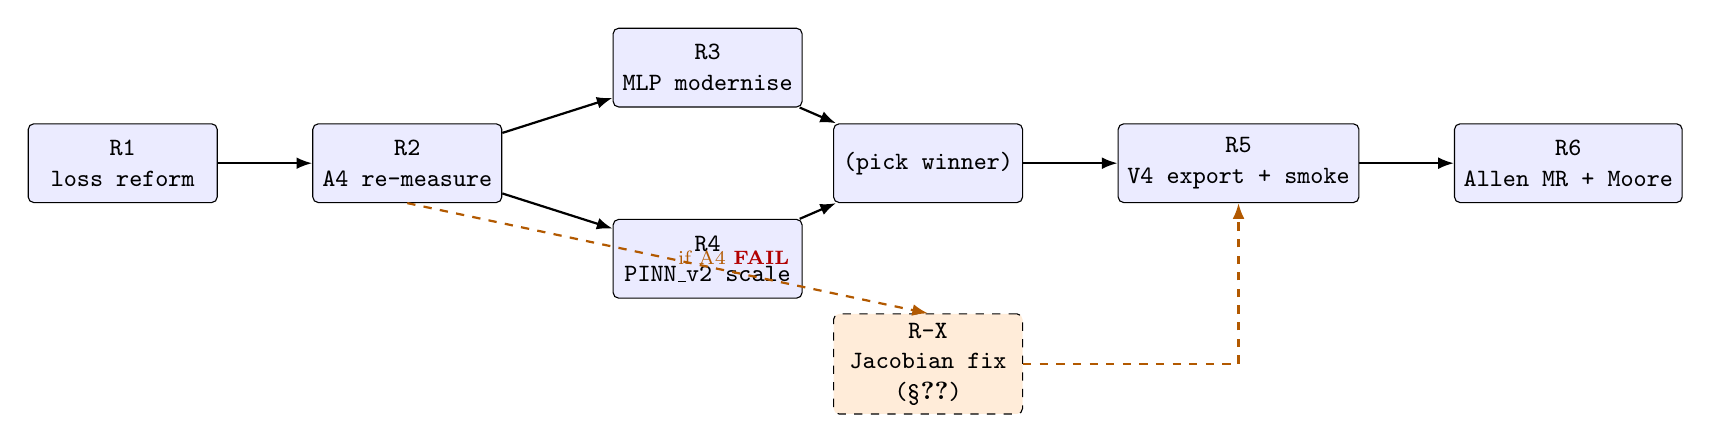
\begin{tikzpicture}[
  node distance=8mm and 12mm,
  phase/.style={draw, rounded corners=2pt, minimum width=24mm,
                minimum height=10mm, font=\small\ttfamily, align=center,
                fill=blue!8},
  rx/.style   ={draw, rounded corners=2pt, minimum width=24mm,
                minimum height=10mm, font=\small\ttfamily, align=center,
                fill=orange!15, dashed},
  arr/.style  ={-{Latex[length=2mm]}, thick}
]
\node[phase] (r1) {R1\\ loss reform};
\node[phase, right=of r1] (r2) {R2\\ A4 re-measure};
\node[phase, above right=2mm and 14mm of r2] (r3) {R3\\ MLP modernise};
\node[phase, below right=2mm and 14mm of r2] (r4) {R4\\ PINN\_v2 scale};
\node[phase, right=42mm of r2] (join) {(pick winner)};
\node[phase, right=of join] (r5) {R5\\ V4 export + smoke};
\node[phase, right=of r5] (r6) {R6\\ Allen MR + Moore};
\node[rx, below=14mm of join] (rx) {R-X\\ Jacobian fix\\ (\S\ref{sec:contingency})};

\draw[arr] (r1) -- (r2);
\draw[arr] (r2) -- (r3);
\draw[arr] (r2) -- (r4);
\draw[arr] (r3) -- (join);
\draw[arr] (r4) -- (join);
\draw[arr] (join) -- (r5);
\draw[arr] (r5) -- (r6);
\draw[arr, dashed, orange!70!black] (r2.south) -- node[right, font=\scriptsize]{if A4 \FAIL} (rx.north);
\draw[arr, dashed, orange!70!black] (rx.east) -| (r5.south);
\end{tikzpicture}
\end{center}

R3 and R4 run in parallel (different model families, no shared
infrastructure). The R-X branch is taken only if Phase~R2 reports A4
failure on both families; in the nominal case it is unused.

% =============================================================================
\section{Concrete merge-request sequence into Allen}
\label{sec:mrs}
% =============================================================================

\subsection{MR-1: \code{!2497} --- already filed}

The current MR places
\code{NRKExtrapolator.cuh} +
\code{NRKExtrapolatorConstants.cuh} +
the \code{m\_use\_nrk} property on \code{extrapolate\_states\_t}.
\textbf{Lands as-is.} The default \code{m\_use\_nrk = false} guarantees
the binary is bytecode-identical to master (ADR~0008 acceptance
criterion). CI throughput retry is the only outstanding gate. No
neural code, no V4 loader, no \code{ITrackExtrapolator} surface change.

\textbf{Files touched.}
\code{Allen/device/kalman/ParKalman/include/NRKExtrapolator.cuh},
\code{Allen/device/kalman/ParKalman/include/NRKExtrapolatorConstants.cuh},
\code{Allen/device/kalman/ParKalman/include/ExtrapolateStates.cuh},
\code{Allen/device/kalman/ParKalman/src/ExtrapolateStates.cu},
\code{Allen/test/unit\_tests/generic/src/TestNRKExtrapolator.cu}.

\subsection{MR-2: V4 blob + \code{forward\_pass} inner loop (after Phase~R5)}

Depends on: Phase~R4 producing a PINN\_v2 winner passing
$< 0.10$\,mm median $|\Delta x|$ and A4
(or the R-X.2 straight-line-residual variant of it).

Adds: V4 schema reader (\code{NeuralWeightsLoader::load\_v4\_blob}),
\code{forward\_pass<ArchTag>} templated specialisations,
\code{NeuralWeights<MLP>} and \code{NeuralWeights<PINN\_V2>} POD types,
a packaged PINN\_v2 \code{.bin} weights file shipped under
\code{Allen/parameters/}. Flips the default in
\code{configuration/python/AllenConf/hlt1\_reconstruction.py} (and
specifically \code{hlt1\_pp\_default.py}) to \code{m\_use\_nrk = True}
with the PINN\_v2 weights as the default blob. The classical RKN4 path
remains under the \code{ArchTag::NRK4} dispatch and the
weights-absent fallback.

\textbf{Files touched (new).}
\code{Allen/device/kalman/ParKalman/include/NeuralWeights.cuh} (new),
\code{Allen/device/kalman/ParKalman/include/ForwardPass.cuh} (new),
\code{Allen/parameters/pinn\_v2\_winner.bin} (new),
plus the V4 spec written into \code{Allen/ML\_research/loader\_v4\_spec.md}.

\textbf{Acceptance gates.}
(i) Unit tests \code{TestNRKExtrapolator.cu} extended with a
\code{TestForwardPass.cu} that compares GPU output to a CPU reference
within $10^{-4}$ relative (A5).
(ii) Standalone Kalman smoke test on a frozen 100-event MDF: per-track
$|\Delta x|$ matches Python reference within ULP-bounds.
(iii) A4 re-measured on the loaded GPU model
\emph{matches} the Python-side measurement (rules out fp32 inference
drift breaking the gate post-load).

\subsection{MR-3: throughput regression + autotune + Moore physics gates (after Phase~R6)}

Depends on: MR-2 merged. \code{allen\_throughput} on the standard
\code{hlt1\_pp\_default} sequence must improve relative to master (A6),
and Moore \code{HltEfficiencyChecker} per-line absolute efficiency loss
must stay $\le 0.5\%$.

Contents: \code{\_\_launch\_bounds\_\_} tuning on
\code{forward\_pass<*>}, fp16 quantisation switch in the loader,
constant$\to$shared promotion if PINN\_v2 width $> [256,256]$,
\code{nsight-compute} regression baselines committed under
\code{Allen/scripts/ci/throughput\_baselines/}.
Moore-side: extend the existing physics-test gate file at
\code{Moore/Hlt/Hlt2Conf/tests/options/hlt2\_track\_efficiency\_pp.py}
to assert the $\le 0.5\%$ envelope.

% =============================================================================
\section*{References}
\addcontentsline{toc}{section}{References}
% =============================================================================

\begin{enumerate}[leftmargin=2em,itemsep=2pt]
\item Canonical goal:
  \href{run:../../PROJECT_CONTEXT.md}{\code{TrackExtrapolation/PROJECT\_CONTEXT.md}}.
\item Replacement plan and constraints A1--A7:
  \href{run:../../experiments/gen_3/REPLACEMENT_PLAN.md}{\code{experiments/gen\_3/REPLACEMENT\_PLAN.md}}
  (\S5, \S6).
\item Off-goal cleanup, \code{NRKExtrapolator.cuh} re-purpose:
  \href{run:../../experiments/gen_3/CLEANUP_LIST.md}{\code{experiments/gen\_3/CLEANUP\_LIST.md}}
  (\S1.3, \S3.6, \S6).
\item Phase structure and V3 loader spec:
  \href{run:../../experiments/gen_3/For_Allen/PLAN.md}{\code{experiments/gen\_3/For\_Allen/PLAN.md}}
  (Phase~0$\to$8; Phase~1b mandatory manifest fields).
\item Current Allen wiring decision (\code{use\_nrk} property,
  \code{ExtrapolateStates} dispatch, deferred Kalman substitution):
  \href{run:../../experiments/gen_3/For_Allen/docs/decisions/0008-allen-wiring-plan.md}{ADR~0008}.
\item Controlling ADR for the replacement goal:
  \href{run:../../experiments/gen_3/For_Allen/docs/decisions/0009-replacement-goal-restated.md}{ADR~0009}.
\item CUDA surface today:
  \href{run:../../../TE_stack/Allen/device/kalman/ParKalman/include/NRKExtrapolator.cuh}{\code{TE\_stack/Allen/device/kalman/ParKalman/include/NRKExtrapolator.cuh}}.
\item Existing Gaudi/Eigen CPU surface (A5 validated for gen-1 MLPs):
  \href{run:../../ml_models/src/TrackMLPExtrapolator.cpp}{\code{ml\_models/src/TrackMLPExtrapolator.cpp}}.
\item Companion theory document:
  \href{run:gen3_replacement_theory_2026-05-19.tex}{\code{gen3\_replacement\_theory\_2026-05-19.tex}}.
\item Companion results document:
  \href{run:gen3_replacement_results_2026-05-19.tex}{\code{gen3\_replacement\_results\_2026-05-19.tex}}.
\item Allen audit (preamble + section conventions matched by this document):
  \href{run:allen_conditions_audit.tex}{\code{docs/reports/allen\_conditions\_audit.tex}}.
\item Allen MR template followed by MR-1:
  \href{https://gitlab.cern.ch/lhcb/Allen/-/merge_requests/2407}{Allen MR !2407}
  (Hoffmann, AdaptiveRKNystromExtrapolator).
\end{enumerate}

\end{document}
